\section{Traffic simulation}
We simulated several vehicles which drive on a set track. All vehicles extend an abstract \texttt{Vehicle} super class. The class diagram for the super and subclasses is seen in figure \ref{fig:ClassDiagram}. The subclasses have fields and methods in common, so we implemented the basic fields and methods in the super class to reduce redundancy.

\begin{figure}[H]
    \centering
    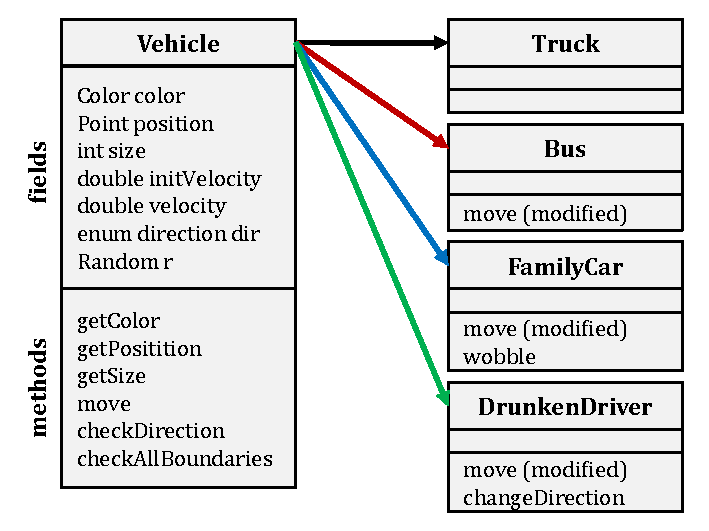
\includegraphics[width=0.7\textwidth]{TrafficSimulation/fig/classDiagram.pdf}
    \caption{Class diagram for \texttt{Vehicle} and its subclasses. \texttt{Truck} is the only vehicle which uses the default \texttt{move} method. All subclasses contain the same fields.}
    \label{fig:ClassDiagram}
\end{figure}

As seen in figure \ref{fig:ClassDiagram} they all extend a template for the \texttt{move} method. This method by default defines a perfectly symmetrical movement counterclockwise around the track. Since all vehicles except \texttt{DrunkenDriver} mainly follows this pattern, it is placed in the super class. The deviations from the default moving pattern is implemented in each subclass. \\
\\
For example: The bus moves like the truck, except in the special case when the bus is in the bottom lane, moving to the right. Hence we implemented the \texttt{move} method in Bus by first calling the \texttt{move} method from \texttt{Vehicle}, and then the special case:

\begin{lstlisting}
public void move() {
// the super class has the default move method used by Truck
super.move();
// if bus is in bottom lane (moving right), move at faster velocity
switch (dir) {
	case RIGHT:
		velocity = 1.6 * initVelocity;
		break;
	default:
		velocity = initVelocity;
...
\end{lstlisting}

\subsection{Collision avoidance}
The \texttt{Vehicle} class also contains some methods to avoid going outside the legal track, as seen on figure \ref{fig:ClassDiagram}. \texttt{checkDirection} is used to check whether a move in the current direction is possible without going outside the track. \\
\texttt{checkAllBoundaries} performs additional checks; it includes checks to keep the vehicle from colliding with the inner ring.\\
\\
All vehicles on the track are shown in figure \ref{fig:traffic1}. As seen on this figure, there is no collision detection between the individual vehicles; they may pass freely through each other. 

\begin{figure}[H]
    \centering
    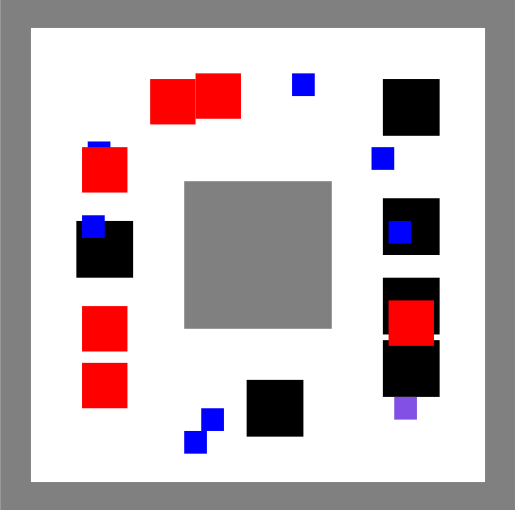
\includegraphics[width=0.7\textwidth]{TrafficSimulation/fig/traffic3}
    \caption{A test run of our traffic simulation.}
    \label{fig:traffic1}
\end{figure}

The subclasses are described in more detail below:

\subsection{\texttt{Truck}}
The \texttt{Truck} subclass is the simplest of all the vehicles. It drives around the track with constant velocity, is the slowest of all vehicles, and the larges. It follows the default move pattern exactly, changing direction when it crosses the center of each corner in a counterclockwise motion.\\

\textbf{Specifications:}
\begin{itemize}
    \item Velocity: 1
    \item Color: Black
    \item Size: 5
\end{itemize}

The \texttt{Truck} should always be the slowest vehicle on the track, so we sets its velocity 
\subsection{\texttt{Bus}}
The \texttt{Bus} and Truck are much alike. The main difference is that the \texttt{Bus}' velocity is not constant on all edges. The \texttt{Bus} speeds up on the bottom edge. 

The \texttt{Bus} is slightly smaller than the \texttt{Truck}, and slightly faster.\\

Specifications:
\begin{itemize}
    \item Velocity: 2 (3 on bottom edge)
    \item Color: \textcolor{red}{Red}
    \item Size: 4
\end{itemize}

\subsection{\texttt{FamilyCar}}
The \texttt{FamilyCar} is more customized than the previous subclasses. It implements the move method from \texttt{Vehicle} but also implements a \texttt{wobble} method which ensures that there is random chance of a deviation from the default moving pattern.\\
\\
The \texttt{FamilyCar} also has a random chance of changing its velocity on each move.
The new velocity is based on the initial velocity (which is preset) and a randomly generated integer.\\

\textbf{Specifications:}
\begin{itemize}
    \item Velocity: 2-4
    \item Color: \textcolor{blue}{Blue}
    \item Size: 2
\end{itemize}

\subsection{\texttt{DrunkenDriver}}
This vehicle is completely chaotic. \texttt{DrunkenDriver} does not use the default movement pattern, so it has a unique \texttt{move} method. As a result, other boundary checking methods were needed.\\
\\
In the beginning of each \texttt{move} method call, the drunk attempts to move forward in its current direction. The new position is checked with one of the boundary checking methods from the \texttt{Vehicle} class. If the drunk would end up inside a wall, it moves backwards instead.\\
\\
\textbf{How the boundary check is performed:}\\
%If this method returns true, the new position is not in danger of colliding with the side or inner walls. 
The method \texttt{checkAllBoundaries} checks whether the position plus vehicle size plus a full step would intersect an illegal area, and returns true of the move is legal. \\

\textbf{Changing directions:}\\
If the \texttt{checkAllBoundaries} returns false, the \texttt{DrunkenDriver} is translated 2 $\cdot$ \texttt{velocity} backwards, and the drunk has a 100 \% chance of choosing a random direction for its next move.\\
\\
After each \texttt{move} method call, no matter if the drunk was close to a wall or not, the \texttt{DrunkenDriver} has a 10 \% chance of choosing a random direction.\\
\\
\textbf{Specifications:}
\begin{itemize}
    \item Velocity: 2-4
    \item Color: Varying color
    \item Size: 2
\end{itemize}


